\documentclass[conference]{IEEEtran}
\IEEEoverridecommandlockouts
% The preceding line is only needed to identify funding in the first footnote. If that is unneeded, please comment it out.
% set language spanish
\usepackage[spanish]{babel}
\usepackage{cite}
\usepackage{amsmath,amssymb,amsfonts}
\usepackage{algorithmic}
\usepackage{graphicx}
\usepackage{textcomp}
\usepackage{xcolor}
\usepackage{hyperref}
\usepackage{caption} 
% center caption
\captionsetup[table]{skip=10pt}
\captionsetup{justification=centering}

\def\BibTeX{{\rm B\kern-.05em{\sc i\kern-.025em b}\kern-.08em
    T\kern-.1667em\lower.7ex\hbox{E}\kern-.125emX}}
\begin{document}

\title{Proyecto 2\\
{\footnotesize \textsuperscript{}Proyecto de clasificación de señas de manos}
\thanks{}
}

\author{\IEEEauthorblockN{1\textsuperscript{st} Sergio Sotil Lozada}
\IEEEauthorblockA{\textit{Estudiante de la carrera de Computer Science} \\
\textit{UTE}\\
201810603 \\
sergio.sotil@utec.edu.pe}
\and
\IEEEauthorblockN{2\textsuperscript{rd} Mario Jacobo Rios Gamboa}
\IEEEauthorblockA{\textit{Estudiante de la carrera de Computer Science} \\
\textit{UTEC}\\
201910285\\
mario.rios@utec.edu.pe}
}

\maketitle

\begin{abstract}
En el presente informe se discutirán los resultados obtenidos luego de clasificar un set de señas de mano a través de los algoritmos:
K-Nearest Neighbors, Support Vector Machine y Decision Tree.
\end{abstract}

\begin{IEEEkeywords}
clasificación,seña de manos, algoritmo
\end{IEEEkeywords}

\section{Introducción}
El código fuente se puede encontrar en \href{https://github.com/morphisjustfun/proyecto_2_AI}{repositorio en Github}. \\
La clasificación es un problema de aprendizaje supervisado que consiste en asignar una etiqueta a un conjunto de datos.
En este caso, se tiene un set de imágenes de señas de manos, las cuales se clasificarán en 24 categorías mediante K-Nearest Neighbors,
Support Vector Machine y Decision Tree. Finalmente, también se validará mediante indicadores cuantitativos y gráficas el desempeño de las técnicas utilizadas.

\section{Explicación de modelos}

\subsection{K-Nearest Neighbors}
Este algoritmo consiste en clasificar un nuevo dato basándose en los K datos más cercanos a él.
Para facilitar este proceso, se emplea una estructura de datos que permita almacenar datos con múltiple dimensionalidad.
Una de las estructuras de datos más utilizadas para este propósito es el árbol KD \ref{fig:kdtree}, el cual permite almacenar datos de múltiples dimensiones de forma eficiente
empleando los mismos principios que un árbol binario.
\begin{figure}[ht]
    \centering
    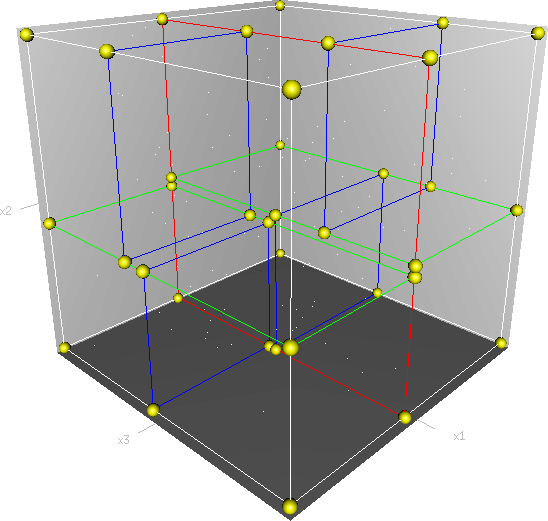
\includegraphics[width=0.25\textwidth]{images/kdtree.png}
    \caption{Árbol KD}
    \label{fig:kdtree}
\end{figure}
\\
De esta forma, se calculan los K vecimos más cercanos y se predice la clase de acuerdo a la clase predominante en los vecinos.
\begin{figure}[ht]
    \centering
    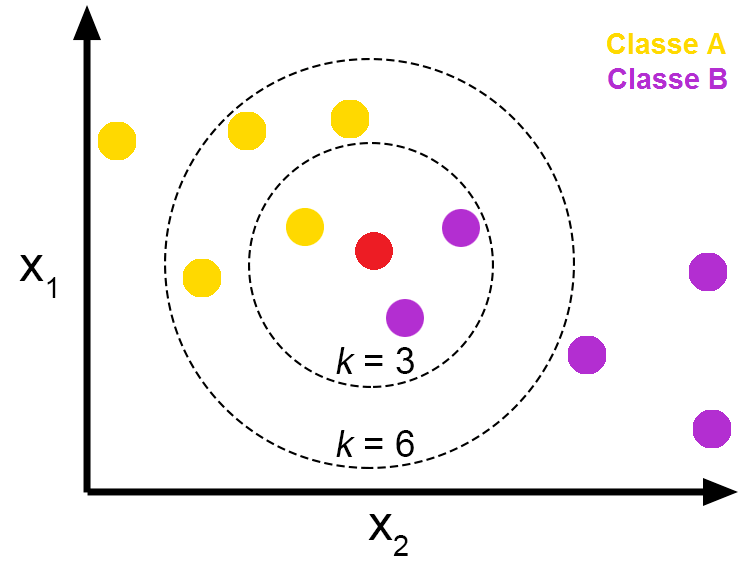
\includegraphics[width=0.25\textwidth]{images/knn.png}
    \caption{Ejemplo de clasificación con K-Nearest Neighbors}
    \label{fig:knn}
\end{figure}

La métrica "distancia"\ puede ser calculada de distintas formas. Entre ellas tenemos a 
la distancia de Manhattan, la cual se calcula sumando las diferencias absolutas de las coordenadas de los puntos.
Otra métrica es la distancia Euclidiana, la cual se calcula sumando las diferencias al cuadrado de las coordenadas de los puntos.
Finalmente, de forma general se tiene la distancia de Minkowski, la cual se calcula elevando a una potencia la suma de las diferencias de las coordenadas de los puntos.
\begin{figure}[ht]
    \centering
    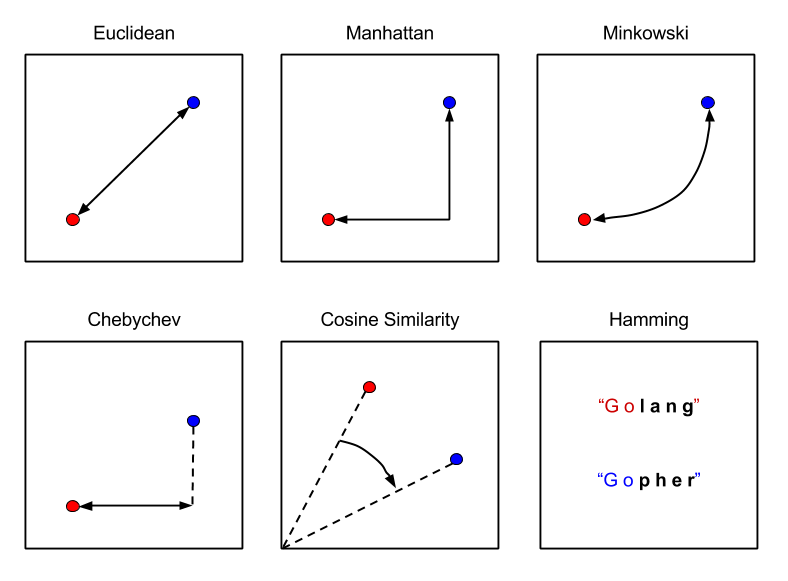
\includegraphics[width=0.40\textwidth]{images/distances.png}
    \caption{Tipos de distancia}
    \label{fig:distance_types}
\end{figure}
\\
En términos de modelado, en una clasificación KNN podemos encontrar los siguientes hiperparámetros:
\begin{itemize}
    \item K: número de vecinos más cercanos a considerar
    \item Tipo de distancia: distancia de Manhattan, distancia Euclidiana o distancia de Minkowski
    \item Estructura de datos: árbol KD, árbol R, árbol R de Hilbert, entre otros
\end{itemize}
\subsection{Support Vector Machine}
Este algoritmo consiste en encontrar un hiperplano que maximice la distancia entre los puntos más cercanos de cada clase.
De esta forma, se puede clasificar un nuevo dato asignándole la clase del lado en el que se encuentre.
\begin{figure}[ht]
    \centering
    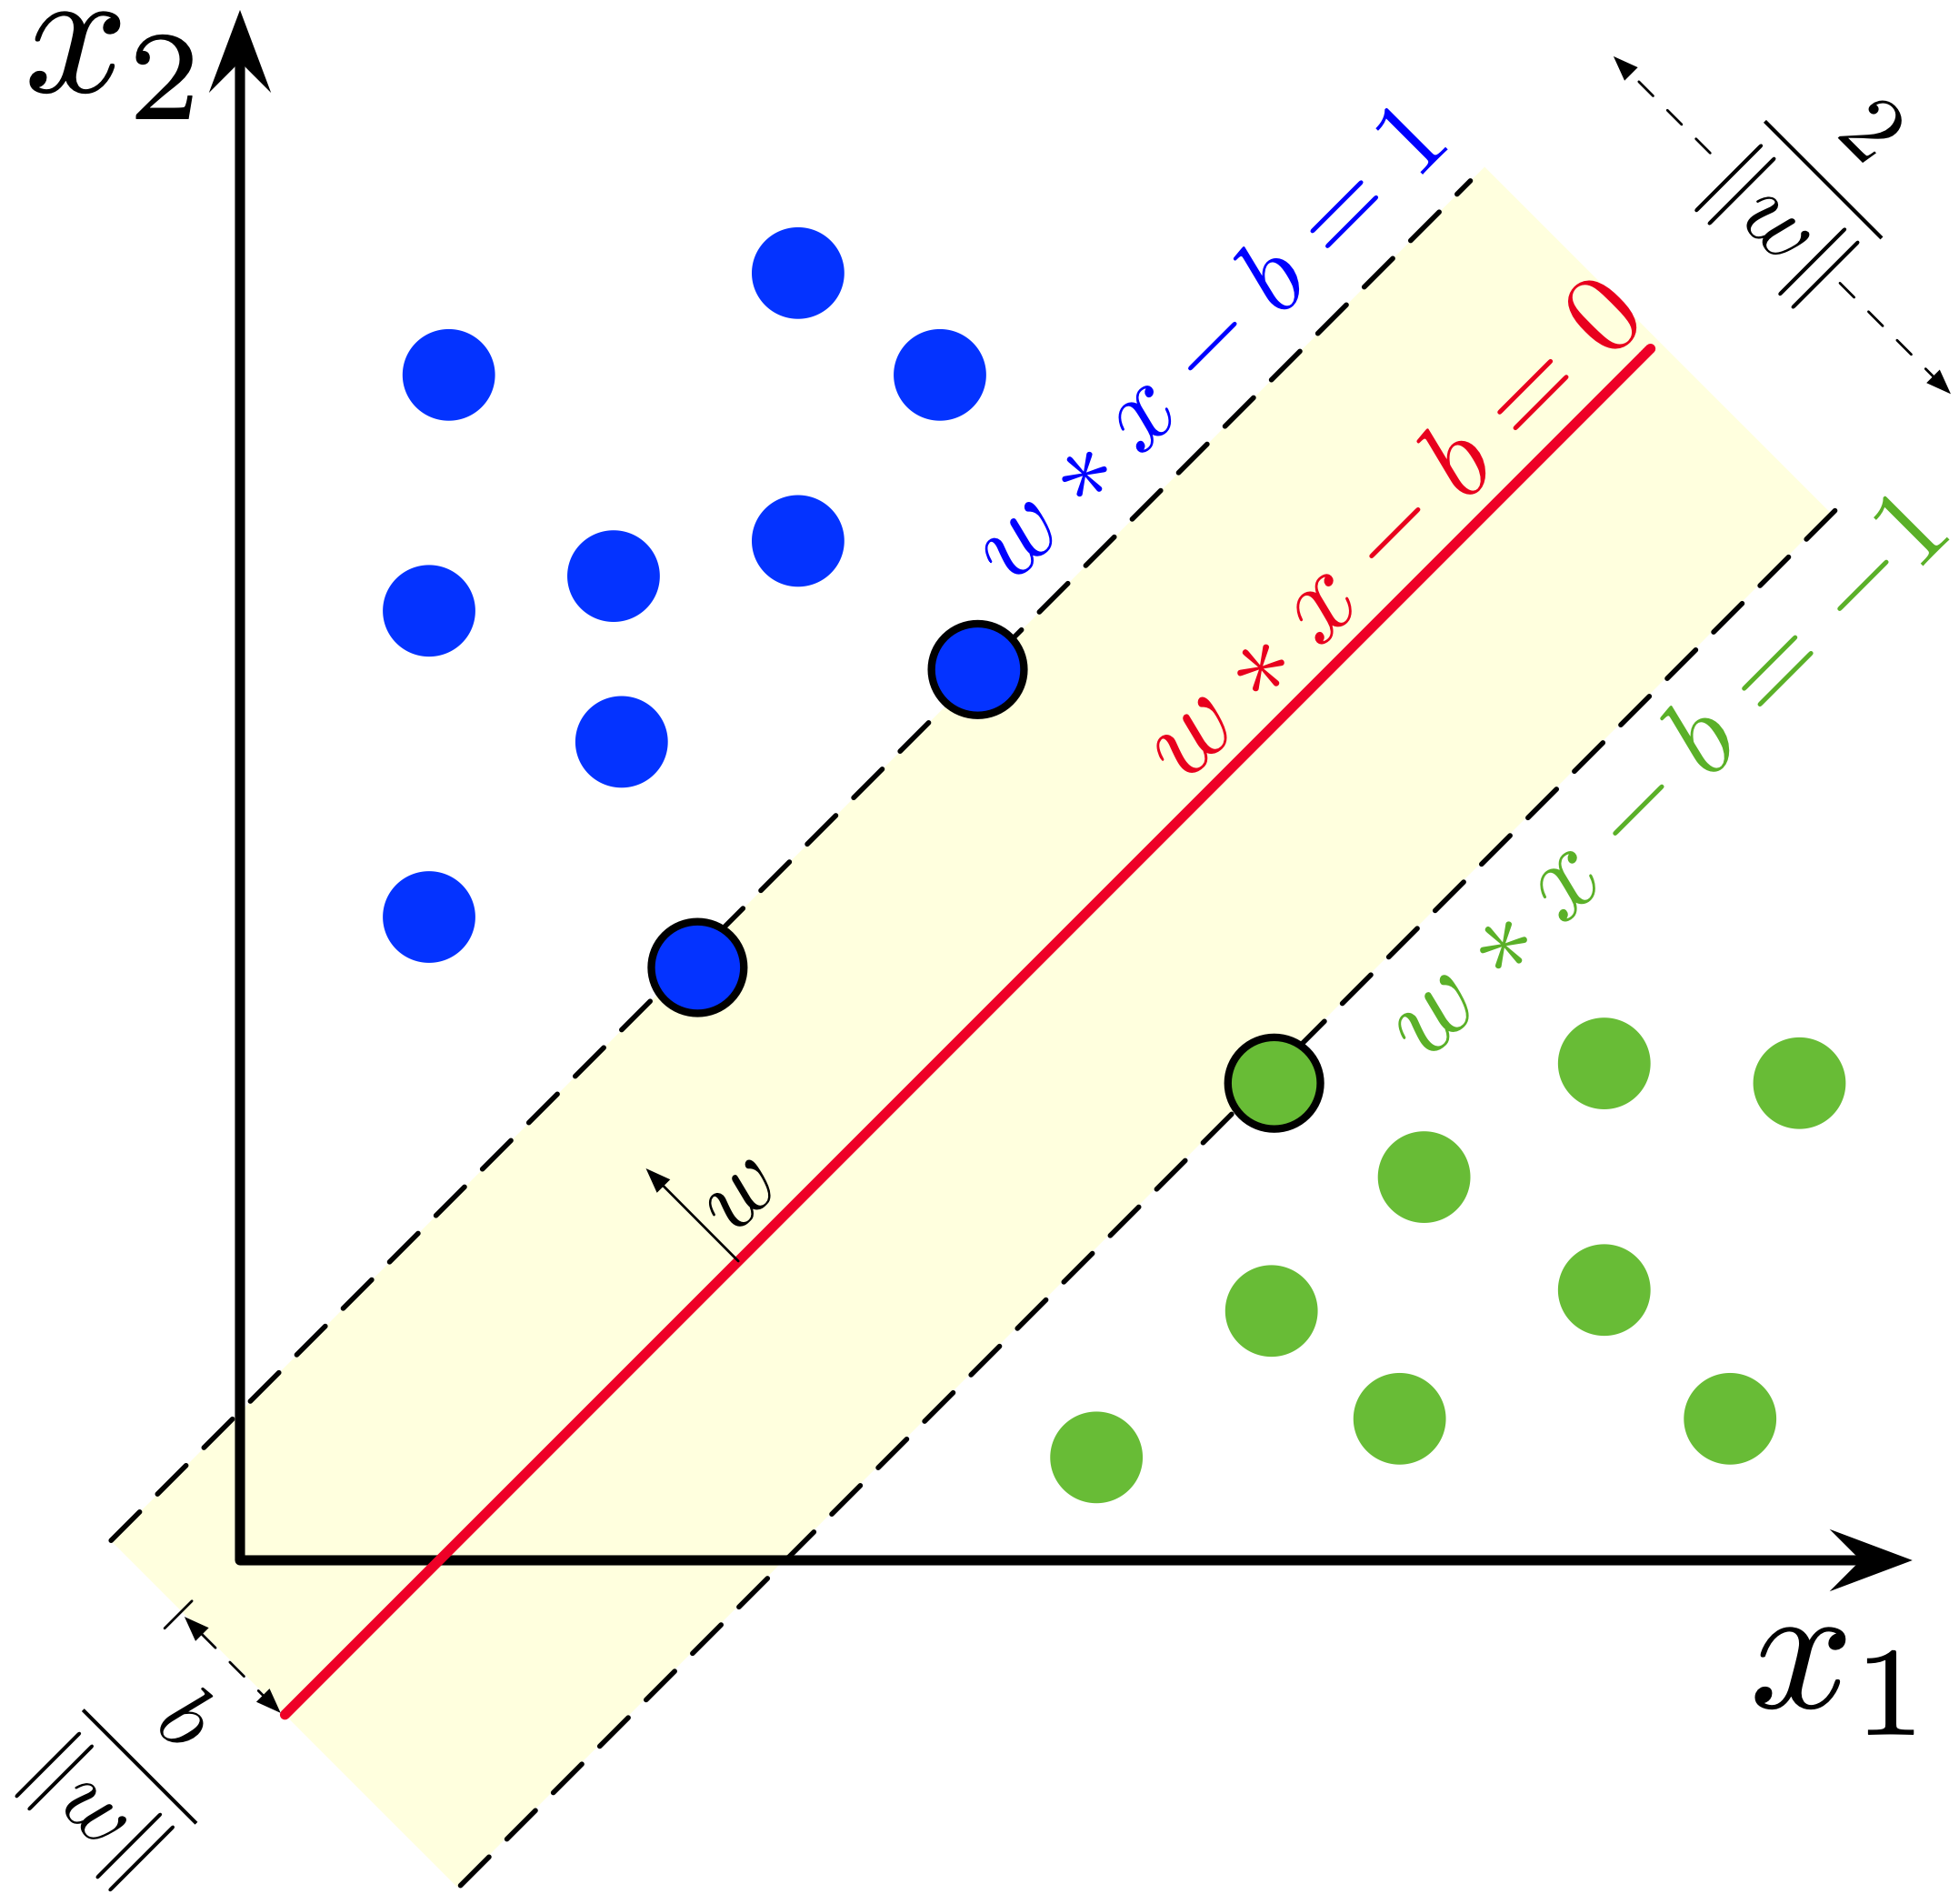
\includegraphics[width=0.25\textwidth]{images/svm.png}
    \caption{Ejemplo de clasificación con Support Vector Machine}
    \label{fig:svm}
\end{figure}
\\
Mientras más largo es el margen del vector de soporte, se reduce potencialmente, el error de generalización del clasificador.
A diferencia de KNN, SVM no requiere de una estructura de datos para almacenar los datos de entrenamiento.

Este algoritmo emplea un kernel para procesar y transformar la data de entrada. Podemos encontrar kernels como:
\begin{itemize}
    \item Kernel Gaussiano
    \item Kernel Polinomial
    \item Kernel RBF (Radial Basis Function)
    \item Kernel Sigmoidal
\end{itemize}
Finalmente, el kernel vendría a ser el principal hiperparámetro que este método emplea.

\subsection{Decision Tree}
Este algoritmo de clasificación emplea la estructura de un árbol. Los nodos internos
representan las características del dataset, las ramas representan las reglas de decisión y cada nodo hoja representa el resultado.
\begin{figure}[ht]
    \centering
    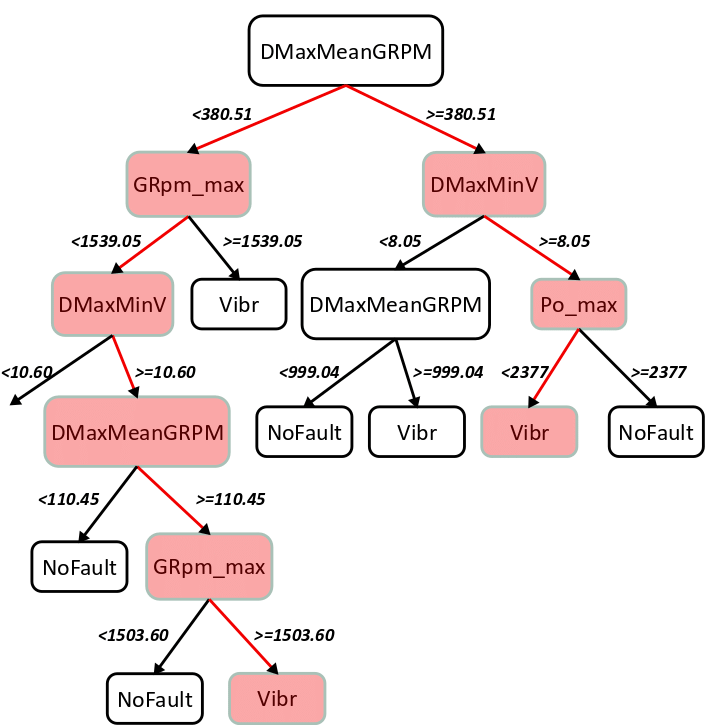
\includegraphics[width=0.25\textwidth]{images/dstree.png}
    \caption{Ejemplo de clasificación con Decision Tree}
    \label{fig:dstree}
\end{figure}
Para entrenar este modelo, se requiere construir el árbol escogiendo en cada nivel una características para partir la información.
Para decidir la mejor característica, se emplea una métrica de impureza. Las métricas más comunes son:
\begin{itemize}
    \item Ganancia de información
    \item Entropía
    \item Gini
\end{itemize}
En caso se tenga una característica continua y numérica se deberá emplear algún criterio para partir los datos, los más comunes son:
\begin{itemize}
    \item Promedio
    \item Mediana
\end{itemize}
Finalmente, para el decision tree podemos encontrar los siguientes hiperparámetros:
\begin{itemize}
    \item Criterio de partición de la data
    \item Métrica de impureza
\end{itemize}
\section{Configuración de entorno y de modelos}
Para todo el proyecto, se empleó el cluster especializado de UTEC - Khipu. El mismo que cuenta con 
la siguiente configuración:

\begin{center}
  \begin{table}[ht]
    \centering
    \begin{tabular}{|c | c | c | c|}
    \hline
    RAM    & N Procesadores & Arquitectura & Sistema operativo \\
    \hline
    126 GB & 80             & x86\_64      & CentOS Linux 7    \\
    \hline
    \end{tabular}
  \end{table}
\end{center}

De los 3 clasificadores propuestos, el Decision Tree y el KNN han sido implementados utilizando el lenguaje
de programación C++. En el Decision Tree se utilizó paralelismo compartido
utilizando la librería OpenMP \ref{fig:openmp}. De esta forma, se reducía de manera considerable
el tiempo de entrenamiento. En efecto, se logró reducir el tiempo de \textbf{2 horas
a 10 minutos} para el dataset entero de \textbf{34627 datos y 784 dimensiones}.


\begin{figure}[ht]
    \centering
    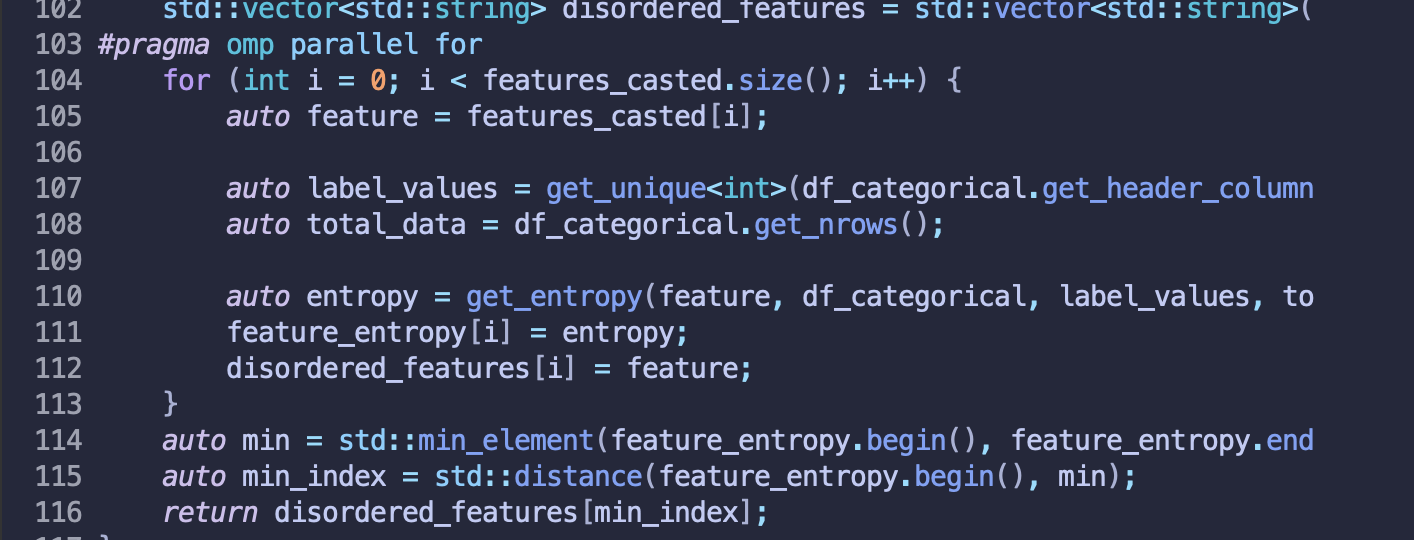
\includegraphics[width=0.35\textwidth]{images/openmp.png}
    \caption{Paralelismo compartido aplicado a el cálculo de la entropía para cada característica}
    \label{fig:openmp}
\end{figure}

En el caso del SVM, se empleó la librería de Python Scikit-learn para entrenar el modelo.
A continuación se detalla más información de la configuración de hiperparámetros de cada modelo:

\begin{itemize}
  \item KDTree
\begin{itemize}
  \item Distancia: Euclidiana
  \item K: Variable entre 1 y 4 (métricas aparte del ROC consideran el caso K = 4)
\end{itemize}

\item SVM
\begin{itemize}
  \item Kernel: RBF
  \item Threshold: Variable dado por la librería
\end{itemize}

\item Decision Tree
\begin{itemize}
  \item Medida de impureza: Entropía
  \item Criterio de partición: Variable entre media y mediana (métricas aparte del ROC
    consideran la media)
\end{itemize}
\end{itemize}

Se emplearán los hiperparámetros variables para generar las curvas ROC. \\
Debido al gran poder de cómputo, no se vio necesario realizar algún tipo de
reducción de dimensionalidad, pues se podía emplear la data completa
en el entrenamiento de los modelos.

\section{Procesamiento de datos}
La base de datos otorgada contaba con \textbf{34627 datos, cada uno de 784 dimensiones (pixeles)}.
La etiqueta de cada dato estaba asignado a la columna 'label' y contaba con un total de 24 valores diferentes.

\begin{figure}[ht]
    \centering
    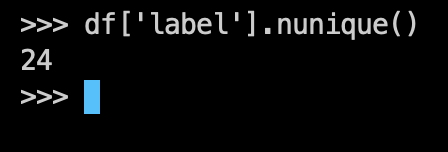
\includegraphics[width=0.35\textwidth]{images/label.png}
    \caption{Distribución de las etiquetas en la base de datos}
    \label{fig:dataset_label}
\end{figure}
\begin{figure}[ht]
    \centering
    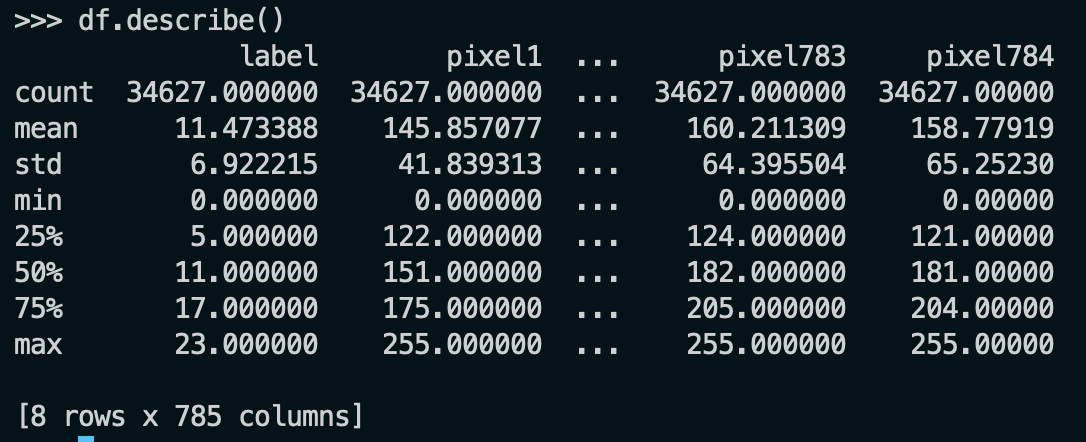
\includegraphics[width=0.35\textwidth]{images/dataset.png}
    \caption{información del dataset}
    \label{fig:dataset_general}
\end{figure}

Primeramente, se notó que en el dataset, la relación de clases estaba desfasada (la clase 9 no existía)
así que se corrigió este error reordenando los valores y sustituyendo los defectuosos.
Seguidamente, se cargó toda la información en memoria y se emplearon 2 técnicas para partir la información y calcular las métricas.

El primer método, KFold Cross Validation, permite dividir el dataset
entero K veces (folds), cada fold tendrá un segmento de datos de training y otros de validación. Esta divisíón se da sin repetición.

El segundo método llamado Bootstraping, realiza un sampling de la información
de manera análoga al KFold, con la diferencia de que este tiene repetición.

En ambos casos, se partió la data entera en 3 folds.

\section{Resultados}

Se emplearon 4 métricas para evaluar el rendimiento de los modelos:
\begin{itemize}
  \item Precisión
  \item Recall
  \item F1 Score
  \item ROC AUC
\end{itemize}

Para el caso de la métrica ROC AUC, se emplearon los hiperparámetros variables para obtener los umbrales.
En el caso de los otros 3 indicadores, se utilizaron las condiciones expuestas con anterioridad.\\
Cabe resaltar que como este es un problema de clasificación de múltiples clases, entonces
para obtener el valor de los indicadores se siguió una estrategia OVR (One vs Rest) lo que implica
que cada característica se evaluó de forma binaria como "Pertenece a la característica" \ o \ "No pertenece a la característica (resto)".\\
Finalmente, se obtuvo el promedio balanceado (weighted) de los valores obtenidos en cada característica. \\

A continuación se muestran los resultados de las métricas para cada modelo
utilizando KFold Cross Validation y Bootstraping:

\begin{center}
  \begin{table}[ht]
    \centering
    \begin{tabular}{|c|c|c|c|c|}
    \hline
    Modelo                 & Precisión & Recall   & F1 score & AUC ROC  \\
    \hline
    SVM & 0.968546  & 0.966672 & 0.966861 & 0.999084 \\
    \hline
    KNN                    & 0.326510  & 0.294539 & 0.299693 & 0.633718 \\
    \hline
    Decision Tree          & 0.775619  & 0.773960 & 0.773440 & 0.861332 \\ 
    \hline
    \end{tabular}
    \caption{Resultados de las métricas para cada modelo utilizando KFold Cross Validation - K = 3}
    \label{tab:results_kfold}
  \end{table}
\end{center}


\begin{center}
  \begin{table}[ht]
    \centering
    \begin{tabular}{|c|c|c|c|c|}
    \hline
    Modelo                 & Precisión & Recall   & F1 score & AUC ROC  \\
    \hline
    SVM & 0.999765  & 0.999765 & 0.999765 & 1.000000 \\
    \hline
    KNN                    & 0.359328  & 0.323336 & 0.330016 & 0.648252 \\
    \hline
    Decision Tree          & 0.856045  & 0.856045 & 0.856161 & 0.902447 \\ 
    \hline
    \end{tabular}
    \caption{Resultados de las métricas para cada modelo utilizando Bootstraping - 3 folds}
    \label{tab:results_bootstrap}
  \end{table}
\end{center}

Se presentan también los mismos resultados a forma de gráfico de barras:

\begin{figure}[ht]
    \centering
    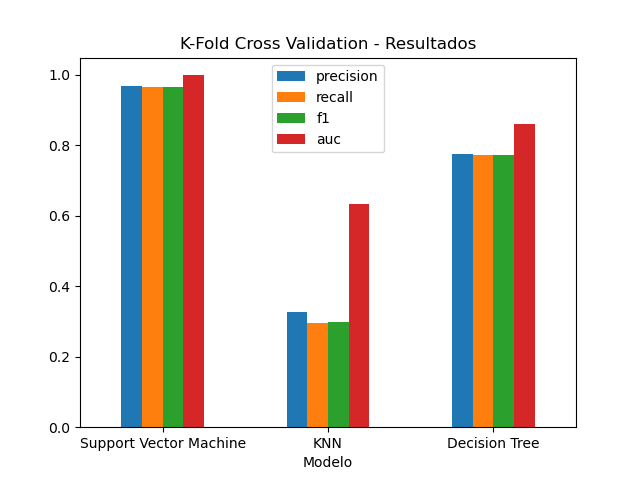
\includegraphics[width=0.35\textwidth]{images/kfold_results.png}
    \caption{Resultados de las métricas para cada modelo utilizando KFold Cross Validation - K = 3}
    \label{fig:kfold_results}
\end{figure}

\begin{figure}[ht]
    \centering
    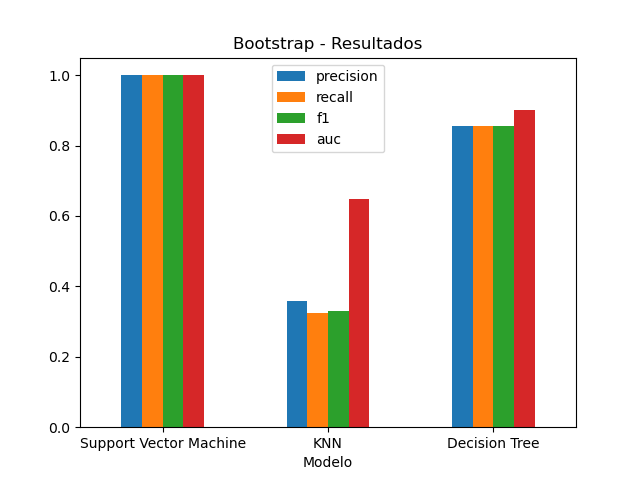
\includegraphics[width=0.35\textwidth]{images/bs_results.png}
    \caption{Resultados de las métricas para cada modelo utilizando Bootstraping - 3 folds}
    \label{fig:bootstrap_results}
\end{figure}

Podemos observar que el modelo SVM obtiene los mejores resultados en todas las métricas, seguido por el Decision Tree y finalmente el KNN.

Una mayor precisión en el modelo SVM implica que dentro de los datos etiquetados como verdaderos. La mayor cantidad
será efectivamente, verdadera. Este atributo es particularmente necesario en la clasificación de señas, pues
mostrarle al usuario una seña incorrecta puede potencialmente alterar el significado de lo que se trataba de expresar.

Por otra parte, el modelo SVM también obtuvo los mejores resultados en cuanto a recall. Esto significa que
de la cantidad de datos que son verdaderos, el modelo SVM es capaz de identificar la mayor cantidad de ellos.

El valor del F1 score es una combinación de precisión y recall, por lo que es una buena métrica para comparar estos dos indicadores
de forma conjunta entre los métodos. No obstante, debido a que el problema consiste
en la identificación de señas, la precisión es más importante que el recall.

La curva ROC nos proporciona una vista gráfica de la relación entre el ratio de falsos positivos con el ratio de verdaderos positivos.
Si el modelo tiene poder predictivo, entonces estará encima de la línea diagonal que pasa por el origen.

A continuación se muestran las curvas ROC para cada modelo en el primer fold de la división KFold Cross Validation:

\begin{figure}[ht]
    \centering
    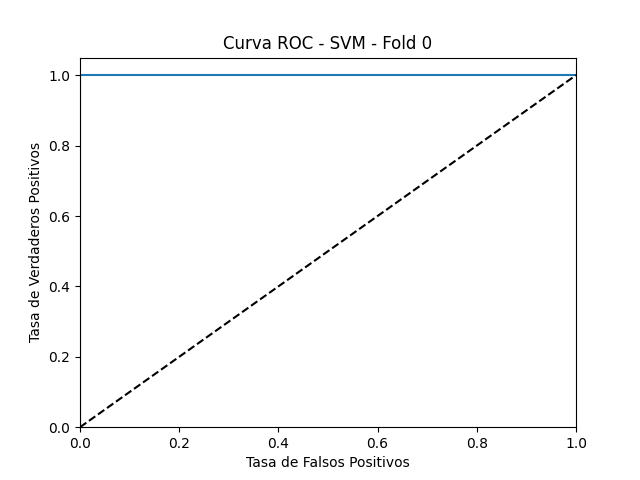
\includegraphics[width=0.35\textwidth]{images/plots/kfold_roc_svm_fold_0.png}
    \caption{Curva ROC para el modelo SVM en el tercer fold de la división KFold Cross Validation}
    \label{fig:kfold_roc_svm_fold_2}
\end{figure}

\begin{figure}[ht]
    \centering
    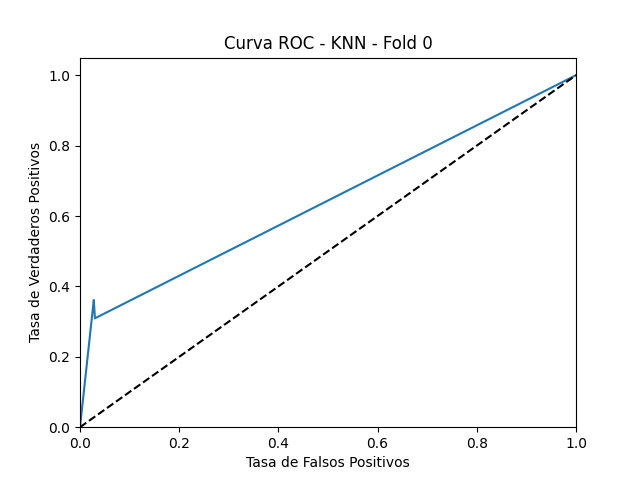
\includegraphics[width=0.35\textwidth]{images/plots/kfold_roc_kdtree_fold0.png}
    \caption{Curva ROC para el modelo KNN en el tercer fold de la división KFold Cross Validation}
    \label{fig:kfold_roc_knn_fold_2}
\end{figure}

\begin{figure}[ht]
    \centering
    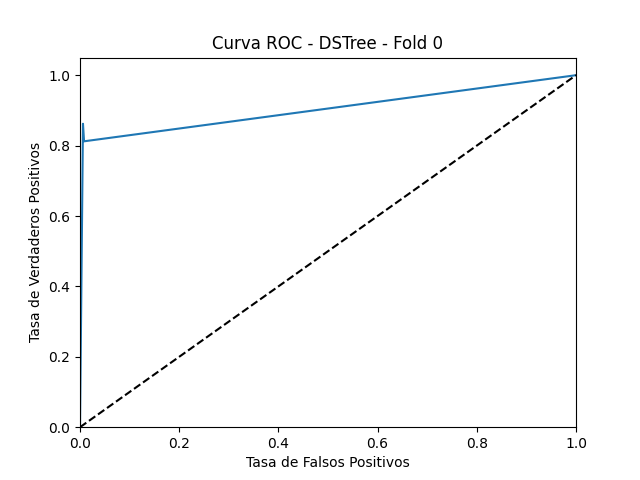
\includegraphics[width=0.35\textwidth]{images/plots/kfold_roc_dstree_fold0.png}
    \caption{Curva ROC para el modelo Decision Tree en el tercer fold de la división KFold Cross Validation}
    \label{fig:kfold_roc_dt_fold_2}
\end{figure}
De las gráficas en conjunto con el valor AUC de las curvas (área) y los indicadores anteriores, concluimos que el clasificador
SVM es el mejor modelo para este problema llegando a comportarse de forma similar a un clasificador perfecto.

El árbol de decisión posee también una fuerte capacidad predictiva. En cuanto al método KNN,
aunque las primeras 3 métricas no son significativas, la curva ROC nos indica que 
tiene cierto poder predictivo y es mejor que un clasificador aleatorio.

\section{Conclusiones}
Se concluye que, el modelo SVM es el mejor para este problema, seguido por el Decision Tree y el KNN.
Para futuras investigaciones, se podría probar variar más hiperparámetros en el Decision Tree como por ejemplo,
el criterio para medir la impureza. Así como el tipo de distancia y la estructura usada en el KNN.
Estructuras como el RTree o el Hilbert RTree permiten indexar de forma más eficiente puntos y objetos multidimensionales facilitando
así la búsqueda de los vecinos más cercanos.
\\
A lo largo del proyecto se ha comprobado como diversos clasificadores se pueden
aplicar a un problema de clasificación de señas. De la misma forma, como distintas
técnicas de evaluación de modelos (muestreos) y métricas explican distintas características
que pueden ser de diferente relevancia de acuerdo a la naturaleza del problema.

\begin{thebibliography}{00}
\bibitem{b1} D. P. Mehta, S. Sahni, ``Handbook of data structures and applications'', CRC Press, 2018.
\bibitem{b2} N. Matloff, ``Statistical Regression and Classification: From Linear Models to Machine Learning'', Chapman and Hall/CRC, 2017.
\end{thebibliography}
\end{document}
